% fs-termtest-A-beamer.tex

\documentclass[xcolor=dvipsnames]{beamer}
\usepackage{teachbeamer}

\title{Term Test A}
\subtitle{{\CourseNumber}, BCIT}

\author{\CourseName}

\date{February 14, 2018}

% \begin{figure}[h]
% 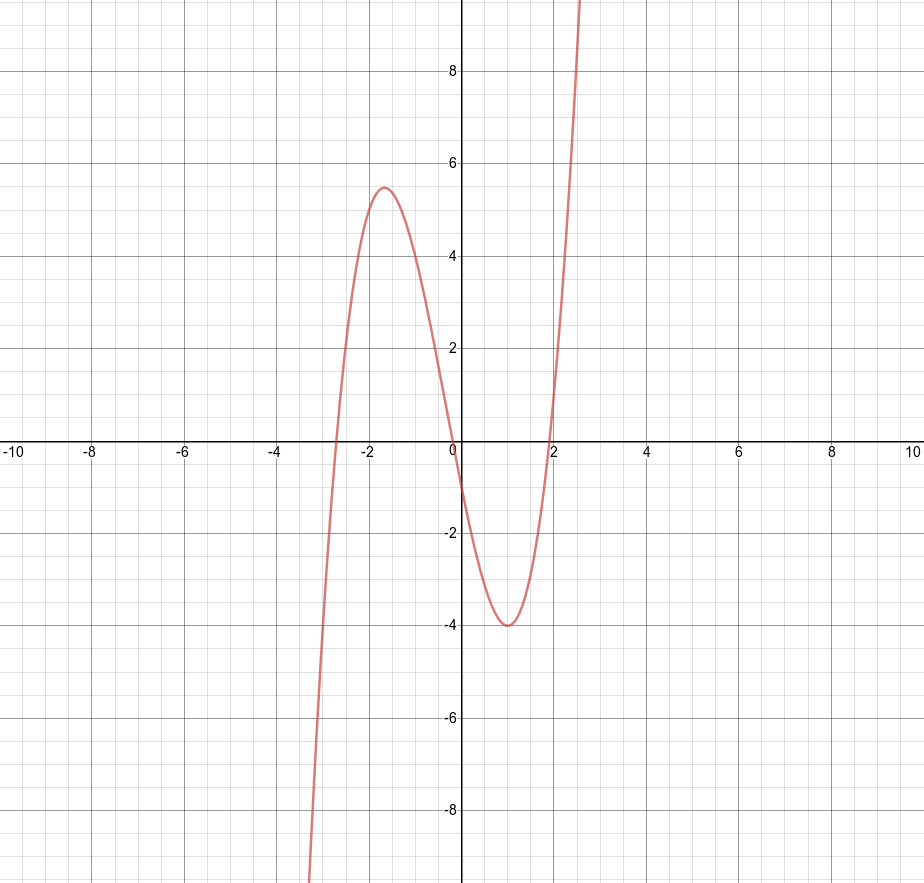
\includegraphics[scale=.3]{./diagrams/extrema1.png}
% \end{figure}

% Command             10pt    11pt    12pt
% \tiny               5       6       6
% \scriptsize         7       8       8
% \footnotesize       8       9       10
% \small              9       10      10.95
% \normalsize         10      10.95   12

\begin{document}

\begin{frame}
  \titlepage
\end{frame}

\begin{frame}
  \frametitle{Term Test A Question 1}
  [6 points] What is the mean and what is the median population of a
  Canadian province/territory? The population numbers in 1000s (census
  2011) are on the next slide.
\end{frame}

\begin{frame}
  \frametitle{Term Test A Question 1}
\begin{tabular}{|l|r|} \hline
Newfoundland and Labrador & 515   \\ \hline
Prince Edward Island      & 140   \\ \hline
Nova Scotia               & 922   \\ \hline
New Brunswick             & 751   \\ \hline
Quebec                    & 7903  \\ \hline
Ontario                   & 12852 \\ \hline
Manitoba                  & 1208  \\ \hline
Saskatchewan              & 1033  \\ \hline
Alberta                   & 3645  \\ \hline
British Columbia          & 4400  \\ \hline
Yukon                     & 34    \\ \hline
Northwest Territories     & 41    \\ \hline
Nunavut                   & 32    \\ \hline
\end{tabular}
\end{frame}

\begin{frame}
  \frametitle{Term Test A Question 2}
[6 points] The father of modern sociology, {\'E}mile Durkheim,
became famous for a study on suicide rates in Catholic and Protestant
countries. Even though you would not be able to predict suicide for
individuals or small groups, on a population level suicide rates are
remarkably stable. Durkheim claimed that the suicide rate is
significantly lower in Catholic populations than in Protestant
populations. Let's assume the suicide rate for Catholics in a given
country and a given year is 0.015\% and the suicide rate for
Protestants is 0.04\%. If this country is predominantly Catholic
(85\%), with 15\% Protestants, then what is the probability that a
person who has committed suicide that year is Catholic?
\end{frame}

\begin{frame}
  \frametitle{Term Test A Question 3}
[6 points] In bag A, there are 4 yellow and 3 green tokens. In bag
B, there are 2 yellow and 5 green tokens. You toss a coin, for which
the probability of heads is 2/3 and the probability of tails is 1/3.
If you toss heads, you draw a token from bag A. If you toss tails, you
draw a token from bag B. What is the probability that you draw a
yellow token?
\end{frame}

\begin{frame}
  \frametitle{Term Test A Question 4}
[4 points] Events $X$ and $\urcorner{}Y$ are independent. Their joint
probability is $0.18$. If $P(Y)=0.4$, then what is $P(X)$?
\end{frame}

\begin{frame}
  \frametitle{Term Test A Question 5}
[6 points] Events $A$ and $B$ are disjoint. If $P(A)=0.2$ and $P(B)=0.4$,
then what is $P(\urcorner{}A\cup\urcorner{}B)$?
\end{frame}

\begin{frame}
  \frametitle{Term Test A Question 6}
[4 points] How many ways are there to draw samples of 5 persons from a
population of 8 persons (order does not matter)?
\end{frame}

\begin{frame}
  \frametitle{Term Test A Question 7}
[6 points] Mother paints 60\% of her Easter eggs green and 40\% in other
colours. Father paints 35\% of his Easter eggs green and 65\% in other
colours. There are one hundred eggs, 62 of which were painted by
Father; the others by Mother. If you find a green egg, what is the
probability that it was painted by Mother?
\end{frame}

\end{document}
